% ==================================================
% CHAPTER 3: Using cosmic muon data for alignment studies
% ==================================================

% Edit count: Lia - 1, Brigitte - 0
\chapter{Using cosmic muon data for alignment studies}

% --------------------------------------------------
\section{Measuring alignment using cosmics data}
% --------------------------------------------------

Misalignments can be modeled as passive transformations. Ideally, a misalignment model would be chosen and the parameters (for example, a global offset and rotation for each layer) calculated. To understand the potential of cosmic muon data, it is useful to define a local offset. For each area of a strip layer, the local offset is the offset of the strip pattern in that area with respect to the nominal geometry.  Local offsets systematically change the strip that is hit by a muon passing through the area. The \package{tgc\_analysis/CosmicsAnalysis} software assumes the nominal geometry, so the recorded muon y-position ($y_{cluster}$) is shifted opposite to the local offset ($d_{local}$),
% Maybe useful sentence?: The local offset is a result of the non-conformities in the strip pattern etching and inter-layer misalignments.
\begin{equation}
    y_{cluster} = y_{nom} - d_{local},
    \label{eqn:local_translation}
\end{equation}
% Maybe useful sentence?: The true position of individual cosmic muons is not known, and in the analysis the four detector planes float with respect to a software-implemented origin that is not associated with a fixed physical location.
where $y_{nom}$ is the position of the muon that would have been recorded if there was no local offset. Equation~\ref{eqn:local_translation} ignores other factors that could affect the cluster position (like resolution). The local offset is unknown and there is no external reference to measure $y_{nom}$. Therefore, only relative alignment parameters can be extracted. 

The minimal relative coordinate system uses two reference or fixed layers~\cite{lefebvre_thesis}. The hits on the two fixed layers were used to create tracks that can be interpolated or extrapolated (polated) to the other two layers. The residual of track $i$, $\Delta_i$ is defined as,
\begin{equation}
    \Delta_i = y_{i,hit} - y_{i,track},
    \label{eqn:residual}
\end{equation}

where $y_{i,hit}$ is the recorded hit position and $y_{i,track}$ is the polated track position built from hits on the two reference layers. Track residuals are affected by the local offset in the area of each layer's hit. As an example, in figure~\ref{fig:fake_event_display}, the residual on layer 2 perhaps indicates that layer 2 is offset with respect to layers 1 and 4 in the area of the track. Of course, a single track residual says nothing of the real relative local offset because of the limited spatial resolution of the detectors and fake tracks caused by noise or delta rays. However, the mean of residuals for all tracks in a region will be shifted systematically by the local offsets between layers~\cite{lefebvre_thesis}. For a perfectly aligned quadruplet, the mean of residuals should be zero in all regions and for all reference frames, unlike the example regions shown in figure~\ref{fig:res_dist}.
\begin{figure}
    \centering
    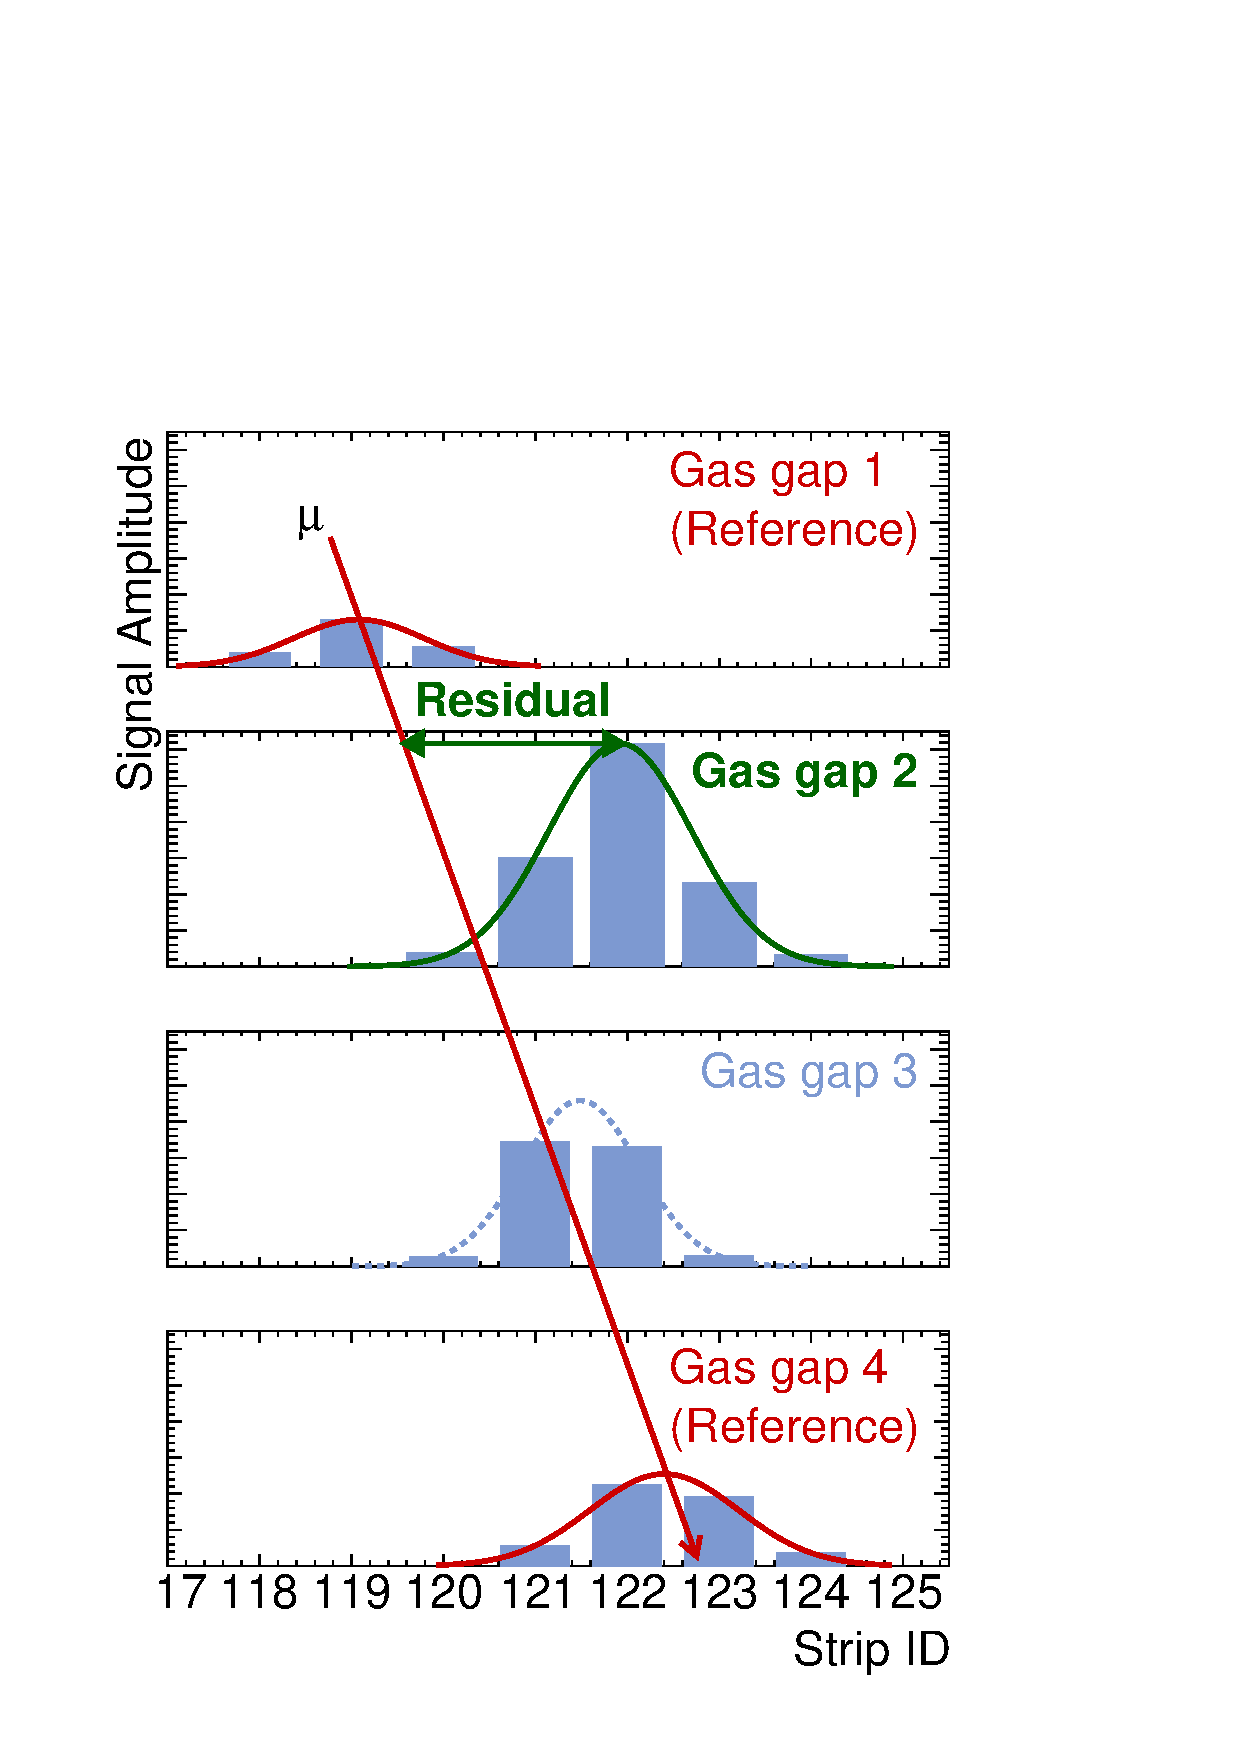
\includegraphics[width = 0.9\textwidth]{figures/figure_fake_event_display.pdf}
    \caption{Representation of a muon event recorded by an sTGC. The clusters are fit with a Gaussian and the mean is taken as the hit position. A track is built from the chosen reference layers, 1 and 4, and the residual calculated on layer 2. The clusters come from a real muon event, but their positions were modified to highlight the idea of residuals.}
    \label{fig:fake_event_display}
\end{figure}

\begin{figure}
\centering
\begin{subfigure}{.5\textwidth}
  \centering
  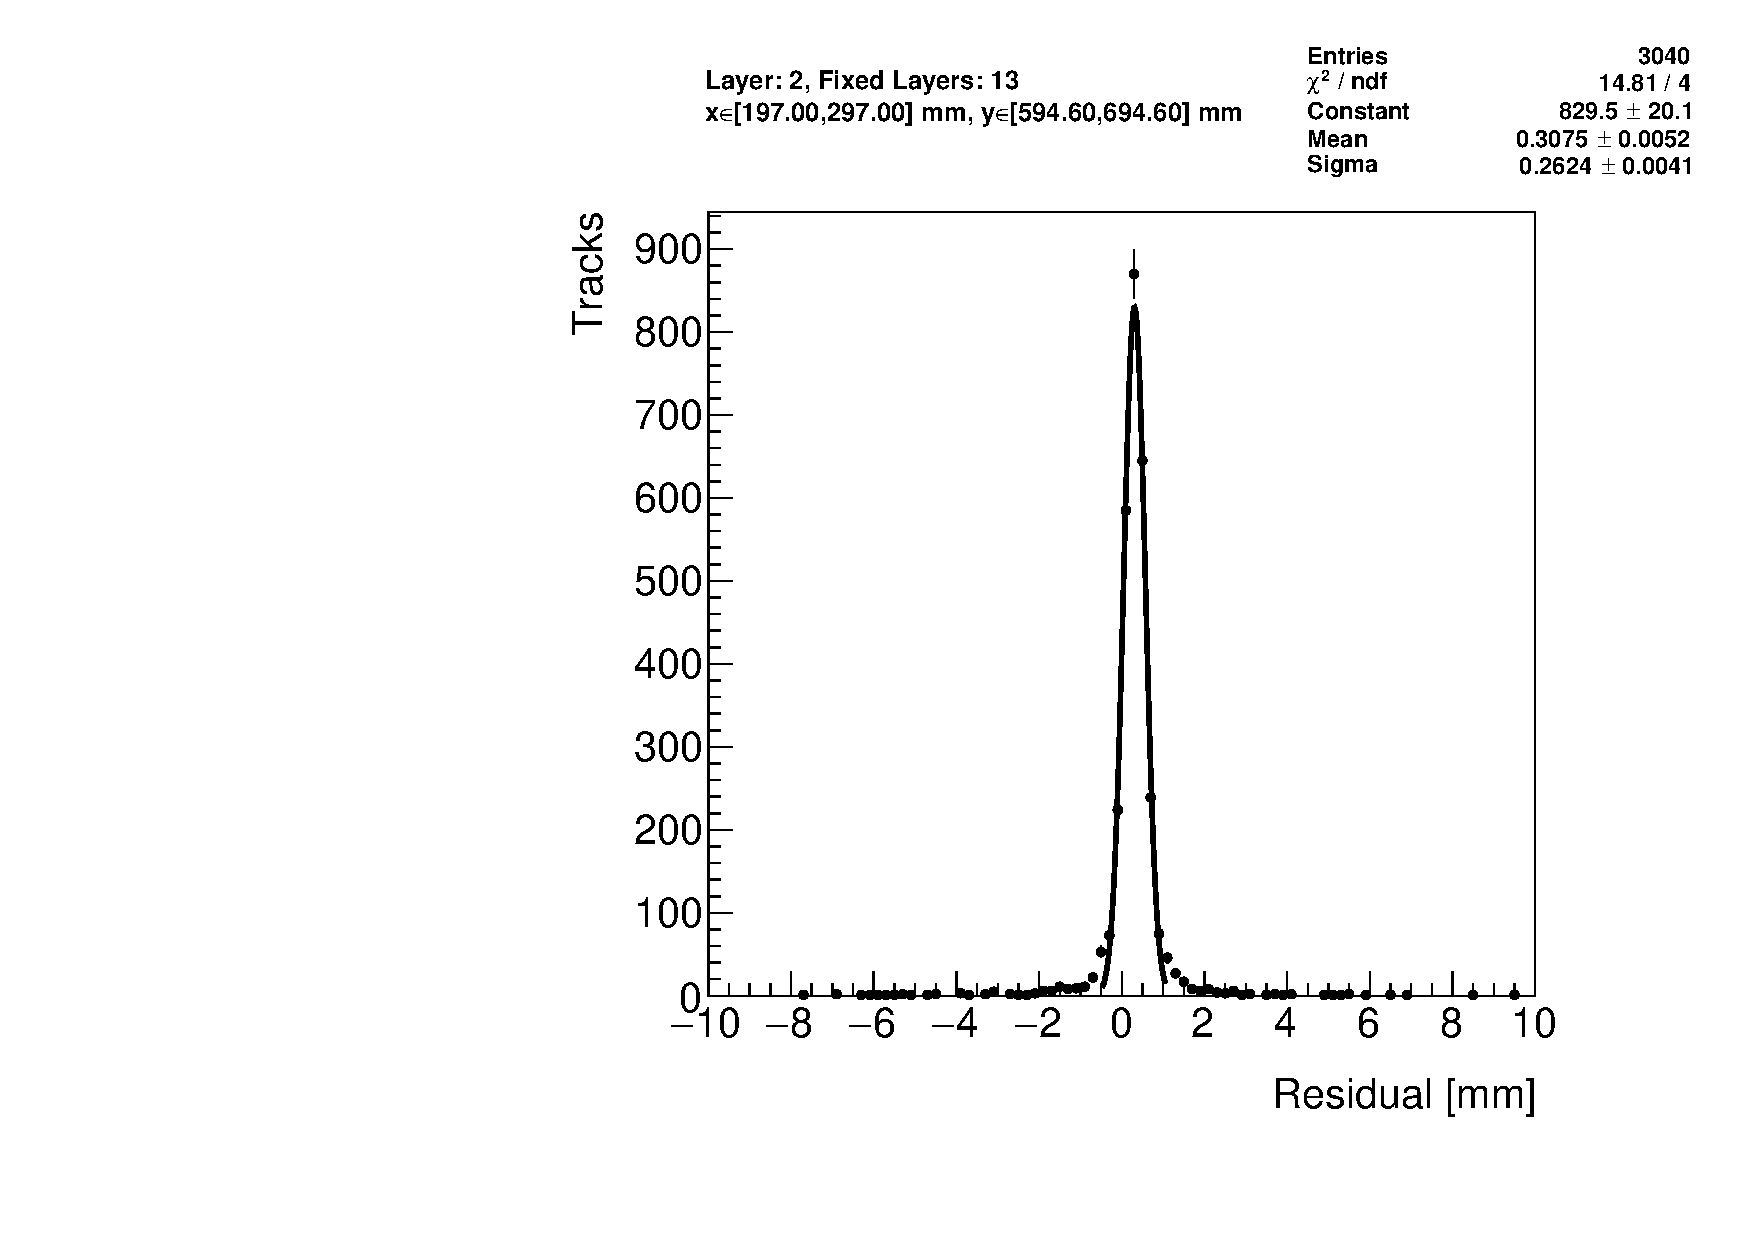
\includegraphics[width=\linewidth]{figures/figure_res_dist_QL2P11_3100V_2021-08-05_xbin_12_ybin_7_layer2_fixedlayers13.pdf}
  \caption{Tracks on layer 2, reference layers 1 and 3.}
  \label{fig:res_dist_L2_F13}
\end{subfigure}%
\begin{subfigure}{.5\textwidth}
  \centering
  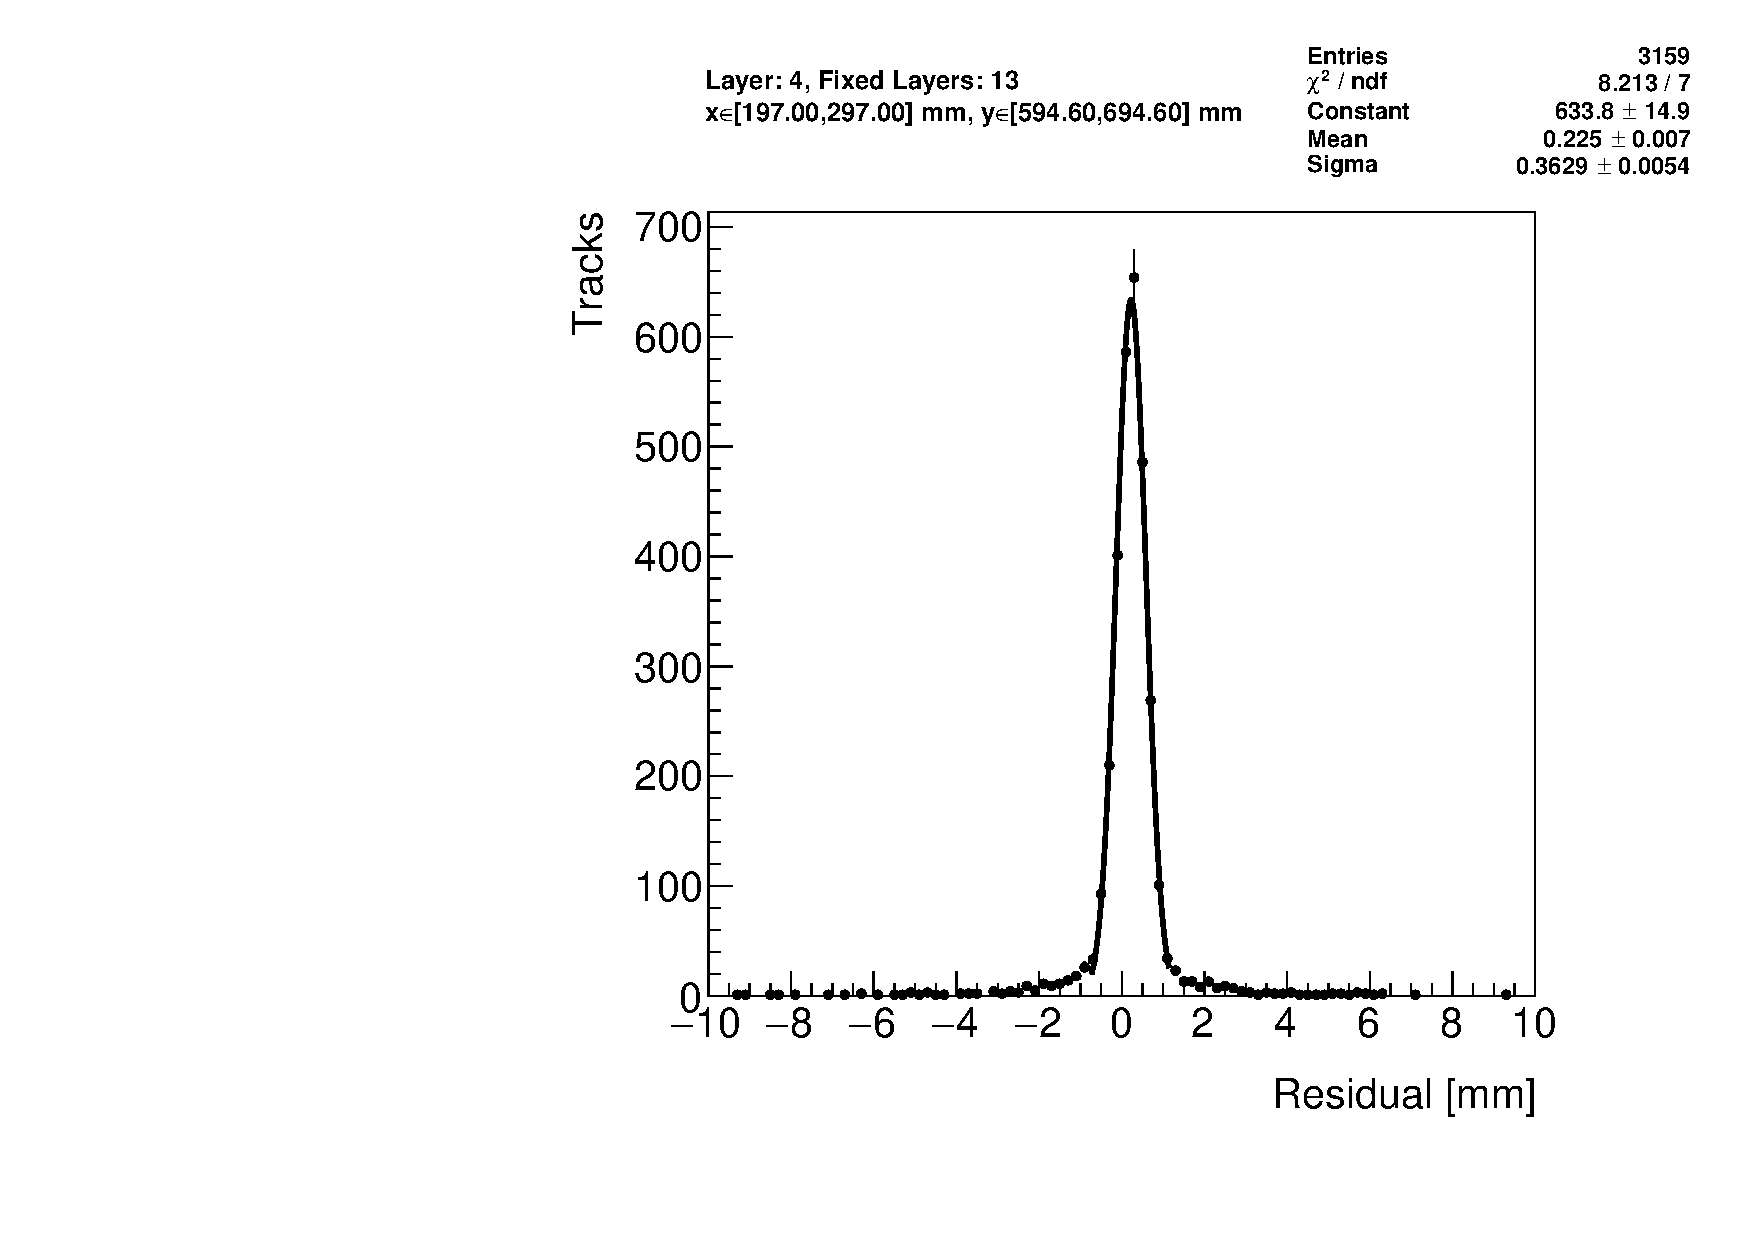
\includegraphics[width=\linewidth]{figures/figure_res_dist_QL2P11_3100V_2021-08-05_xbin_12_ybin_7_layer4_fixedlayers13.pdf}
  \caption{Tracks on layer 4, reference layers 1 and 2.}
  \label{fig:res_dist_L4_F12}
\end{subfigure}
\caption{Residual distribution in the region $x\in\left[197, 297\right],  y\in\left[594.6, 694.6\right] mm$ (100 mm by 100 mm area) for two different tracking combinations. }
\label{fig:res_dist}
\end{figure}

The residual distributions were wider for tracking combinations where the extrapolation lever arm was largest. In general, residual means calculated with geometrically less favourable tracking combinations have larger statistical and systematic uncertainties. The bin size of \SI{200}{\micro\meter} for the distributions shown in figure~\ref{fig:res_dist} was chosen based on the uncertainty on residuals calculated from tracks on layer 4 (1) built from hits on layers 1 and 2 (3 and 4) given a cluster y-position uncertainty of \SI{60}{\micro\meter} (\ref{appendix:clustering}), since these tracks yield residuals with the largest uncertainties.

A gaussian fit was used to extract the mean of the residual distributions. Theoretically, a double gaussian distribution is more apt, but for this analysis the gaussian fit was sufficient, as discussed in appendix~\ref{appendix:systematics_res_fit_fcn}.

The motivation for the area of the region of interest will be discussed in CHAPTER 5, COMPARISON (ADD IN REF ONCE CREATED).

It is only possible to calculate relative local offsets with csomics data because there was no external reference which positions on all layers could be measured with respect to. As an example, in figure~\ref{fig:fake_event_display}, the residual on layer 2 could be caused by layer 2 being misaligned from nominal, but it could also be caused by layers 1 and 4 being misaligned from nominal while layer 2 is in its expected position! Any number of combinations of local offsets on layers 1, 2 and 4 could produce the residual on layer 2. Nonetheless, the value of relative local offset measurements will be shown and discussed throughout this work.

% --------------------------------------------------
\section{Visualizing relative misalignments between layers}
% --------------------------------------------------

The mean of residuals was extracted for regions across entire quadruplet layers for every tracking combination to get a picture of the relative misalignments between layers. 

\begin{figure}
\centering
\begin{subfigure}{0.85\textwidth}
  \centering
  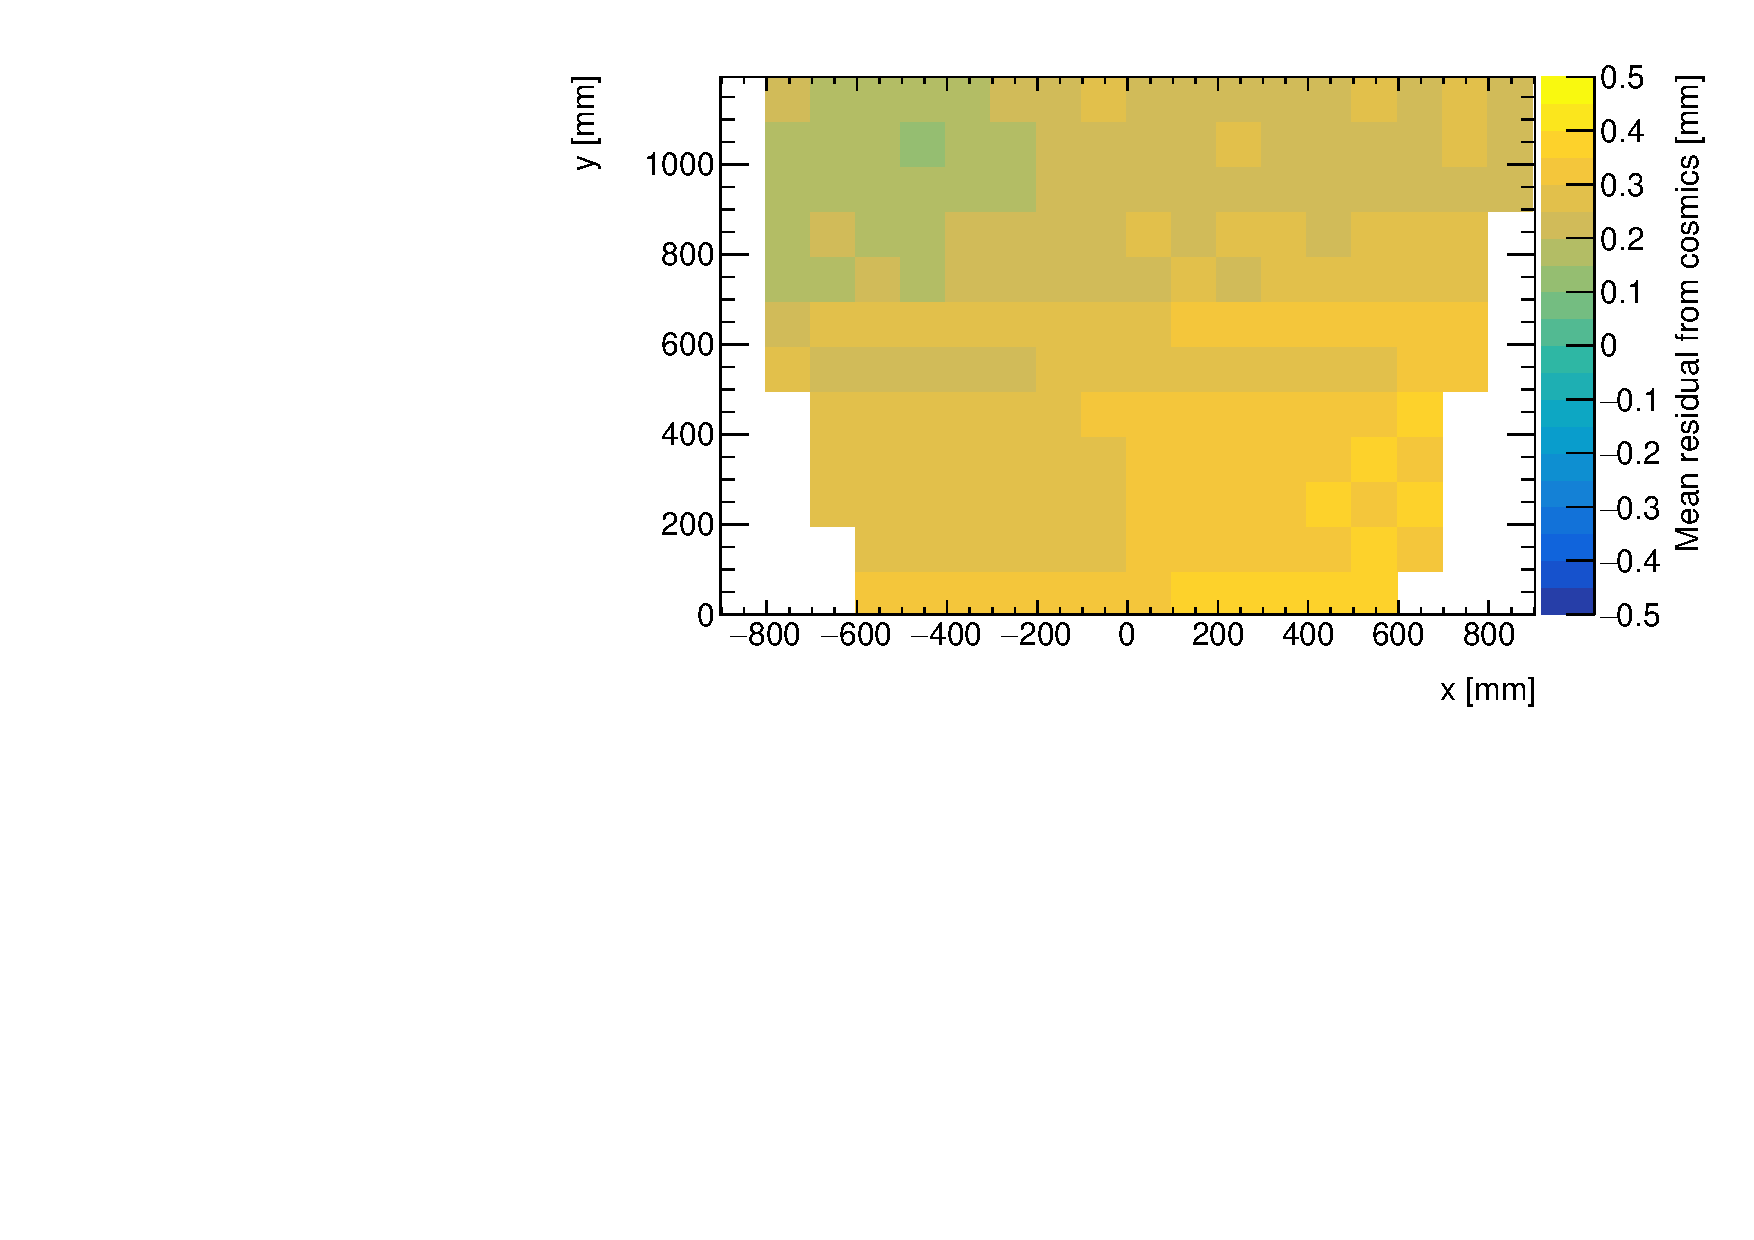
\includegraphics[width=\linewidth]{figures/figure_QL2P11_3100V_2021-08-05_th2_means_layer2_fixedlayers13.pdf}
  \caption{Mean of residuals for tracks on layer 2, reference layers 1 and 3.}
  \label{fig:res_mean_th2_L2_F13}
\end{subfigure}%
\vspace*{\floatsep}
\begin{subfigure}{0.85\textwidth}
  \centering
  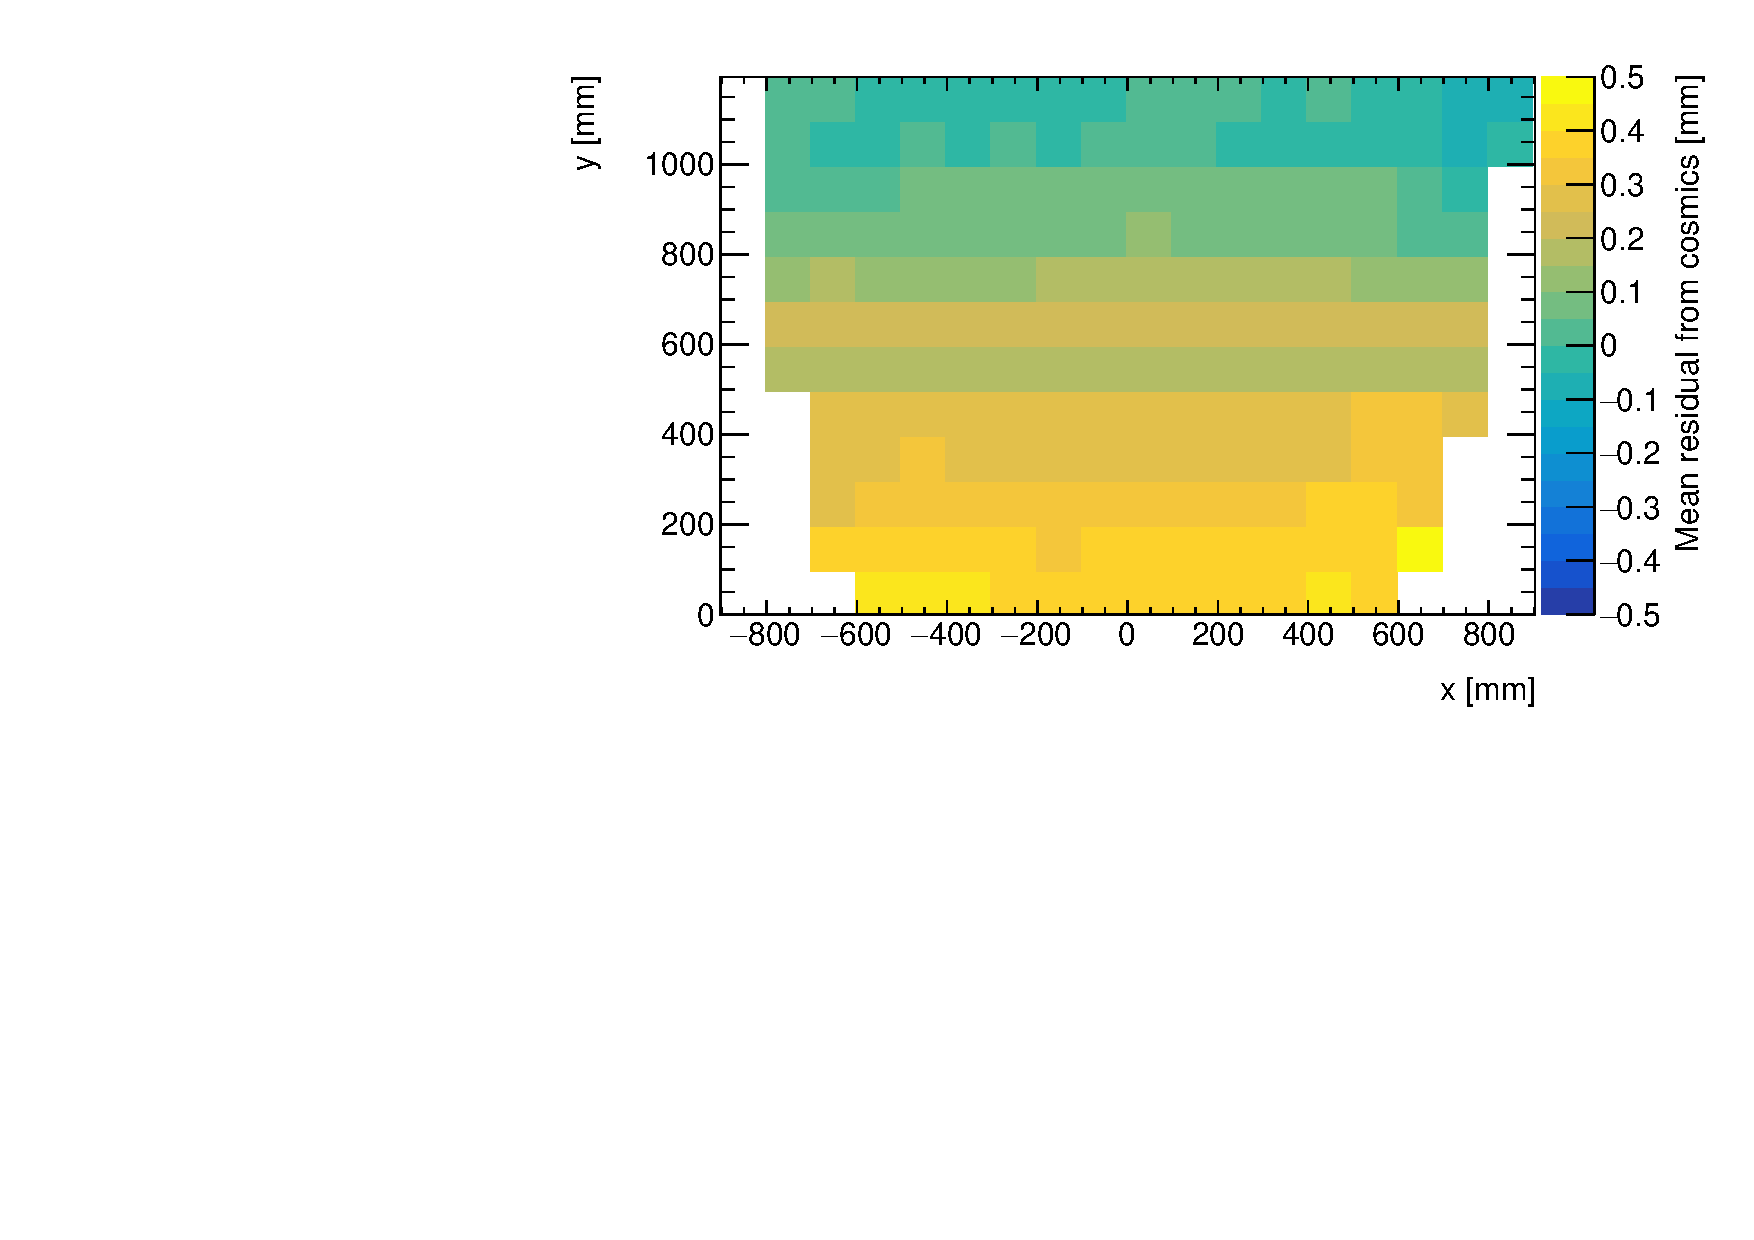
\includegraphics[width=\linewidth]{figures/figure_QL2P11_3100V_2021-08-05_th2_means_layer4_fixedlayers13.pdf}
  \caption{Mean of residuals for tracks on layer 4, reference layers 1 and 3.}
  \label{fig:res_mean_th2_L4_F13}
\end{subfigure}
\caption{Mean of residuals in each \SI{100}{\milli\meter} by \SI{100}{\milli\meter} bin over the area of the quad layer.}
\label{fig:res_mean_th2}
\end{figure}

Figure~\ref{fig:res_mean_th2}, contains the mean of residuals on layers 2 and 4 with tracking reference layers 1 and 3. Many of the residual means are non-zero, indicating that there are local relative misalignments. Given that the residual mean changes with $x$ in figure~\ref{fig:res_mean_th2_L2_F13}, there is likely a rotation of layer 2 with respect to layers 1 and 3, combined with an offset of the entire layer. For layer 4 in figure~\ref{fig:res_mean_th2_L4_F13}, perhaps there is a scaling~\cite{carlson_results_2019} of the strip pattern with respect to layers 1 and 3. The interpretation of the patterns in the residual means depends on the choice of misalignment model.

Work on characterizing relative misalignments between quadruplet layers in ongoing~\cite{zhao_cosmic_2019}, \textcolor{red}{(Can I cite John's thesis-in-progress?)} but what is required are the absolute strip positions with respect to their nominal position in the ATLAS analysis coordinate system \textcolor{red}{to be input into Athena(?)}. Somehow, absolute misalignment parameters must be derived to create a model of absolute strip positions - which is not possible with the cosmics dataset. Absolute local offset measurements were done by the so-called x-ray method, discussed in CHAPTER 4 X-RAY METHOD (REF ONCE CREATED). Given the degree of confidence in the local mean cosmic residual measurements detailed below, they were used to validate the absolute local offset measurements provided by the x-ray method (details to follow in CHAPTER 5 COMPARISON).

% --------------------------------------------------
\section{Systematic uncertainty}
% --------------------------------------------------

The statistical uncertainty on the local residual means was typically around \SI{10}{} - \SI{20}{\micro\meter}, and appendix~\ref{appendix:statistics} shows that the analysis was not statistically limited by the number of triggers collected for each quadruplet. The systematic uncertainties were more significant. 

Systematic uncertainties were assigned per tracking combination as the RMS of the distribution of the difference in local residual means calculated each with a different analysis choice. For example, the RMS associated with fitting the local residual distributions with a Gaussian or double Gaussian is \SI{25}{\micro\meter} for the geometrically least favourable tracking combinations and the distribution is shown in appendix~\ref{appendix:systematics_res_fit_fcn}. For geometrically similar tracking combinations (like: tracks on layer 1 built from hits on layers 3 and 4, and tracks on layer 4 built from hits on layers 1 and 2), the systematic uncertainty was assigned as the average RMS for both.

Other choices were whether to use data collected at 2.9~kV or 3.1~kV; what cluster fitting algorithm to use; and whether or not to apply a differential non-linearity (DNL) correction to the cluster y-positions. A systematic uncertainty was assigned using the method above to account for the effect of each choice. The reasons for each choice are listed below.

Data taken at 3.1~kV was used over 2.9~kV because the strip and wire tracking efficiency increases with higher voltage~\cite{lefebvre_thesis} (appendix~\ref{appendix:systematics_2900V_vs_3100V}).

The \package{Minuit2} package~\cite{hatlo_developments_2005} was used to fit clusters over Guo's method~\cite{guo_simple_2011} because it provided automatic statistical uncertainty estimates and is the standard choice (appendix~\ref{appendix:systematics_cluster_fit_fcn}).

The DNL correction was not applied because its effect on the residual means was negligible (appendix~\ref{appendix:systematics_dnl}).

A summary of the systematic uncertainties assigned for each tracking combination is given in table~\ref{tab:sys_uncerts}.

%TODO : Maybe just make the table have the total sys uncertainty, and put the breakdown at the end of appendix:systematics
%\begin{center}
\begin{table}

\begin{tabularx}{\textwidth} {
 | >{\raggedright\arraybackslash}X 
 | >{\raggedright\arraybackslash}X 
 | >{\raggedright\arraybackslash}X
 | >{\raggedright\arraybackslash}X 
 | >{\raggedright\arraybackslash}X 
 | >{\raggedright\arraybackslash}X 
 | >{\raggedright\arraybackslash}X 
 | >{\raggedright\arraybackslash}X 
 | >{\raggedright\arraybackslash}X | }
 
 \hline
 \textbf{Layer} & \textbf{Fixed layer 1} & \textbf{Fixed layer 2} & \textbf{\ref{appendix:systematics_res_fit_fcn}} & \textbf{\ref{appendix:systematics_2900V_vs_3100V}} & \textbf{\ref{appendix:systematics_cluster_fit_fcn}} & \textbf{\ref{appendix:systematics_dnl}} & \textbf{Total} \\ 
 \hline
 \hline 
 3 & 1 & 2 & 0.010 & 0.041 & 0.018 & 0.008 & \textbf{0.047} \\
 \hline
    4 & 1 & 2 & 0.025 & 0.091 & 0.027 & 0.012 & \textbf{0.098} \\
 \hline
    2 & 1 & 3 & 0.008 & 0.020 & 0.012 & 0.003 & \textbf{0.025} \\
 \hline
    4 & 1 & 3 & 0.007 & 0.042 & 0.013 & 0.005 & \textbf{0.044} \\
 \hline
    2 & 1 & 4 & 0.006 & 0.035 & 0.012 & 0.005 & \textbf{0.038} \\
 \hline
    3 & 1 & 4 & 0.006 & 0.035 & 0.012 & 0.005 & \textbf{0.038} \\
 \hline
    1 & 2 & 3 & 0.010 & 0.041 & 0.018 & 0.008 & \textbf{0.047} \\
 \hline
    4 & 2 & 3 & 0.010 & 0.041 & 0.018 & 0.008 & \textbf{0.047} \\
 \hline
    1 & 2 & 4 & 0.007 & 0.042 & 0.013 & 0.005 & \textbf{0.044} \\
 \hline
    3 & 2 & 4 & 0.008 & 0.020 & 0.012 & 0.003 & \textbf{0.025} \\
 \hline
    1 & 3 & 4 & 0.025 & 0.091 & 0.027 & 0.012 & \textbf{0.098} \\
 \hline
    2 & 3 & 4 & 0.010 & 0.041 & 0.018 & 0.008 & \textbf{0.047} \\
 \hline
 
\end{tabularx}
\caption{Systematic uncertainty assigned for each analysis option, detailed in appendix~\ref{appendix:systematics}.}
\label{tab:sys_uncerts}
\end{table}

Given that the uncertainty in the cosmics residual means is lesser than or near to the order of the required position resolution of the sTGCs (\SI{100}{\micro\meter}~\cite{nsw_tdr} the cosmic residual means are relevant for characterizing misalignments.






